%!TEX program = xelatex
\documentclass{beamer}

%\usepackage{pgfpages}
%\setbeameroption{show notes}
\setbeamerfont{note page}{size=\tiny}
%\setbeameroption{show notes on second screen}

\usepackage{booktabs}
\usepackage{pifont}
\usepackage{wasysym}
\usepackage{amsmath}
\usepackage{rotating}
\usepackage{appendixnumberbeamer}
\usepackage[caption=false]{subfig}
\usepackage{siunitx}
\usepackage{xfrac}
\usepackage{pgfplots}
\pgfplotsset{compat=newest}
\usepackage{pgfplotstable}
\usetikzlibrary{plotmarks,arrows}
\tikzset{>=latex}

\usetheme{Execushares}

\title{Numerical Characterization of Ultrasound Elastography for the Early Detection of Deep Tissue Injuries}
\subtitle{A thesis submitted in partial fulfilment of the requirements for the degree of Master of Science}
\author{Kenton David Hamaluik}
\institute{University of Alberta}
\date{June 23, 2014}

\newcommand{\rotHead}[1]{\begin{rotate}{60}#1\end{rotate}}
\newcommand{\cmark}{\color{ExecusharesBlue}\ding{51}}
\newcommand{\xmark}{\color{ExecusharesRed}\ding{55}}
\newcommand{\percent}{\%}

\pgfmathdeclarefunction{gauss}{3}{%
  \pgfmathparse{1/(#2*sqrt(2*pi))*exp(-((#3-#1)^2)/(2*#2^2))}%
}

\definecolor{pc1}{HTML}{8DD3C7}
\definecolor{pc2}{HTML}{FDB462}
\definecolor{pc3}{HTML}{FB8072}
\definecolor{pc4}{HTML}{80B1D3}
\definecolor{pc5}{HTML}{B3DE69}
\definecolor{pc6}{HTML}{BEBADA}
\definecolor{pc7}{HTML}{FCCDE5}
\definecolor{pc8}{HTML}{D9D9D9}
\definecolor{pc9}{HTML}{FFFFB3}

\pgfplotscreateplotcyclelist{ColourPlotCycle}{%
only marks,mark options=solid,solid,thick,pc1,every mark/.append style={fill=pc1},mark=*\\%
only marks,mark options=solid,solid,thick,pc2,every mark/.append style={fill=pc2},mark=square*\\%
only marks,mark options=solid,solid,thick,pc3,every mark/.append style={fill=pc3},mark=diamond*\\%
only marks,mark options=solid,solid,thick,pc4,every mark/.append style={fill=pc4},mark=pentagon*\\%
only marks,mark options=solid,solid,thick,pc5,every mark/.append style={fill=pc5},mark=triangle*\\%
only marks,mark options=solid,solid,thick,pc6,every mark/.append style={fill=pc6},mark=*\\%
only marks,mark options=solid,solid,thick,pc7,every mark/.append style={fill=pc7},mark=square*\\%
only marks,mark options=solid,solid,thick,pc8,every mark/.append style={fill=pc8},mark=diamond\\%
only marks,mark options=solid,solid,thick,pc9,every mark/.append style={fill=pc9},mark=pentagon\\%
}

\pgfplotscreateplotcyclelist{ColourPlotRegressionCycle}{%
only marks,solid,thick,pc1,every mark/.append style={fill=pc1},mark options=solid,mark=*\\%
solid,thick,pc1\\%
only marks,solid,thick,pc2,every mark/.append style={fill=pc2},mark options=solid,mark=square*\\%
solid,thick,pc2\\%
only marks,solid,thick,pc3,every mark/.append style={fill=pc3},mark options=solid,mark=diamond*\\%
solid,thick,pc3\\%
only marks,solid,thick,pc4,every mark/.append style={fill=pc4},mark options=solid,mark=pentagon*\\%
solid,thick,pc4\\%
only marks,solid,thick,pc5,every mark/.append style={fill=pc5},mark options=solid,mark=triangle*\\%
solid,thick,pc5\\%
only marks,solid,thick,pc6,every mark/.append style={fill=pc6},mark options=solid,mark=*\\%
solid,thick,pc6\\%
only marks,solid,thick,pc7,every mark/.append style={fill=pc7},mark options=solid,mark=square\\%
solid,thick,pc7\\%
only marks,solid,thick,pc8,every mark/.append style={fill=pc8},mark options=solid,mark=diamond\\%
solid,thick,pc8\\%
only marks,solid,thick,pc9,every mark/.append style={fill=pc9},mark options=solid,mark=pentagon\\%
solid,thick,pc9\\%
}

\pgfplotscreateplotcyclelist{SmoothColourPlotCycle}{%
solid,ultra thick,pc1\\%
solid,ultra thick,pc2\\%
solid,ultra thick,pc3\\%
solid,ultra thick,pc4\\%
solid,ultra thick,pc5\\%
solid,ultra thick,pc6\\%
solid,ultra thick,pc7\\%
solid,ultra thick,pc8\\%
solid,ultra thick,pc9\\%
}

\pgfplotscreateplotcyclelist{BarColourPlotCycle}{%
fill=pc1\\%
fill=pc2\\%
fill=pc3\\%
fill=pc4\\%
fill=pc5\\%
fill=pc6\\%
fill=pc7\\%
fill=pc8\\%
fill=pc9\\%
}

\definecolor{RdBuWhiteGrey}{RGB}{247,247,247}
\pgfplotsset{
	colormap={RdBu}{
		rgb255(0cm)=(5,48,97);
		rgb255(1cm)=(33,102,172);
		rgb255(2cm)=(67,147,195);
		rgb255(3cm)=(146,197,222);
		rgb255(4cm)=(209,229,240);
		rgb255(5cm)=(247,247,247);
		rgb255(6cm)=(253,219,199);
		rgb255(7cm)=(244,165,130);
		rgb255(8cm)=(214,96,77);
		rgb255(9cm)=(178,24,43);
		rgb255(10cm)=(103,0,31);
	}
}

\pgfplotsset{
	colormap={YlOrRd}{
		rgb255(0cm)=(128,0,38);
		rgb255(1cm)=(189,0,38);
		rgb255(2cm)=(227,26,28);
		rgb255(3cm)=(252,78,42);
		rgb255(4cm)=(253,141,60);
		rgb255(5cm)=(254,178,76);
		rgb255(6cm)=(254,217,118);
		rgb255(7cm)=(255,237,160);
		rgb255(8cm)=(255,255,204);
	}
}
% for drawing legends with regressions
\newcommand{\drawLegendMarks}[1]{
	\addlegendimage{empty legend}
	\addlegendimage{solid,thick,pc1,every mark/.append style={fill=pc1},mark options=solid,mark=*}
	\ifnum#1>1
		\addlegendimage{solid,thick,pc2,every mark/.append style={fill=pc2},mark options=solid,mark=square*}
	\fi
	\ifnum#1>2
		\addlegendimage{solid,thick,pc3,every mark/.append style={fill=pc3},mark options=solid,mark=diamond*}
	\fi
	\ifnum#1>3
		\addlegendimage{solid,thick,pc4,every mark/.append style={fill=pc4},mark options=solid,mark=pentagon*}
	\fi
	\ifnum#1>4
		\addlegendimage{solid,thick,pc5,every mark/.append style={fill=pc5},mark options=solid,mark=triangle*}
	\fi
	\ifnum#1>5
		\addlegendimage{solid,thick,pc6,every mark/.append style={fill=pc6},mark options=solid,mark=*}
	\fi
	\ifnum#1>6
		\addlegendimage{solid,thick,pc7,every mark/.append style={fill=pc7},mark options=solid,mark=square*}
	\fi
	\ifnum#1>7
		\addlegendimage{solid,thick,pc8,every mark/.append style={fill=pc8},mark options=solid,mark=diamond}
	\fi
	\ifnum#1>8
		\addlegendimage{solid,thick,pc9,every mark/.append style={fill=pc9},mark options=solid,mark=pentagon}
	\fi
	\addlegendimage{dashed,ExecusharesGrey}
}

\DeclareDocumentCommand\characterizationPlots{ m m g g g g }{%
	\addplot+[forget plot,dashed,mark=none,draw=ExecusharesGrey,sharp plot] coordinates { (0,0) (3.5,3.5) };
	\addplot+[forget plot] table{../latex/assets/#2}; \pgfplotsset{cycle list shift=1};%
	\addplot+[forget plot] table[y={create col/linear regression={y=#1}}] {../latex/assets/#2}; \pgfplotsset{cycle list shift=2};%
	\xdef\slopeA{\pgfplotstableregressiona}; \xdef\interA{\pgfplotstableregressionb};%
	\IfNoValueF {#3} {%
		\addplot+[forget plot] table{../latex/assets/#3}; \pgfplotsset{cycle list shift=3};%
		\addplot+[forget plot] table[y={create col/linear regression={y=#1}}] {../latex/assets/#3}; \pgfplotsset{cycle list shift=4};%
		\xdef\slopeB{\pgfplotstableregressiona}; \xdef\interB{\pgfplotstableregressionb};%
	}%
	\IfNoValueF {#4} {%
		\addplot+[forget plot] table{../latex/assets/#4}; \pgfplotsset{cycle list shift=5};%
		\addplot+[forget plot] table[y={create col/linear regression={y=#1}}] {../latex/assets/#4}; \pgfplotsset{cycle list shift=6};%
		\xdef\slopeC{\pgfplotstableregressiona}; \xdef\interC{\pgfplotstableregressionb};%
	}%
	\IfNoValueF {#5} {%
		\addplot+[forget plot] table{../latex/assets/#5}; \pgfplotsset{cycle list shift=7};%
		\addplot+[forget plot] table[y={create col/linear regression={y=#1}}] {../latex/assets/#5}; \pgfplotsset{cycle list shift=8};%
		\xdef\slopeD{\pgfplotstableregressiona}; \xdef\interD{\pgfplotstableregressionb};%
	}%
	\IfNoValueF {#6} {%
		\addplot+[forget plot] table{../latex/assets/#6}; \pgfplotsset{cycle list shift=9};%
		\addplot+[forget plot] table[y={create col/linear regression={y=#1}}] {../latex/assets/#6}; \pgfplotsset{cycle list shift=10};%
		\xdef\slopeD{\pgfplotstableregressiona}; \xdef\interD{\pgfplotstableregressionb};%
	}%
}

\DeclareDocumentCommand\comparisonPlots{ m }{%
	\addplot+[forget plot,dashed,mark=none,draw=ExecusharesGrey,sharp plot] coordinates { (0,0) (3.5,3.5) };
	\pgfplotstableread{../latex/assets/conclusions/#1.dat}{\tableData};%
	\addplot+[forget plot] table[x={trueSR}, y={quasiSR}] {\tableData}; \pgfplotsset{cycle list shift=1};%
	\addplot+[forget plot] table[y={create col/linear regression={y=quasiSR}}] {\tableData}; \pgfplotsset{cycle list shift=2};%
	\xdef\slopeA{\pgfplotstableregressiona}; \xdef\interA{\pgfplotstableregressionb};%
	\addplot+[forget plot] table[x={trueSR}, y={arfiSR}] {\tableData}; \pgfplotsset{cycle list shift=3};%
	\addplot+[forget plot] table[y={create col/linear regression={y=arfiSR}}] {\tableData}; \pgfplotsset{cycle list shift=4};%
	\xdef\slopeB{\pgfplotstableregressiona}; \xdef\interB{\pgfplotstableregressionb};%
	\addplot+[forget plot] table[x={trueSR}, y={shearSR}] {\tableData}; \pgfplotsset{cycle list shift=5};%
	\addplot+[forget plot] table[y={create col/linear regression={y=shearSR}}] {\tableData}; \pgfplotsset{cycle list shift=6};%
	\xdef\slopeC{\pgfplotstableregressiona}; \xdef\interC{\pgfplotstableregressionb};%
}%

\DeclareDocumentCommand\characterizationLegend{ m m m g g g g}{%
	\drawLegendMarks{\IfNoValueTF{#7}{\IfNoValueTF{#6}{\IfNoValueTF{#5}{\IfNoValueTF{#4}{1}{2}}{3}}{4}}{5}};%
	\addlegendentry{\tiny\textbf{#1}};%
	\addlegendentry{$#2 = #3$};%
	\IfNoValueF {#4} { \addlegendentry{$#2 = #4$}; }%
	\IfNoValueF {#5} { \addlegendentry{$#2 = #5$}; }%
	\IfNoValueF {#6} { \addlegendentry{$#2 = #6$}; }%
	\IfNoValueF {#7} { \addlegendentry{$#2 = #7$}; }%
	\addlegendentry{\tiny Unary Mapping}
	%
	%\addlegendentry{\textbf{#1}};%
	%\addlegendentry{$#2 = #3$, $E_{rel,meas} = \pgfmathprintnumber[fixed,fixed zerofill,precision=2]{\slopeA} E_{rel,nom} \pgfmathprintnumber[print sign,fixed,fixed zerofill,precision=2]{\interA}$};%
	%\IfNoValueF {#4} { \addlegendentry{$#2 = #4$, $E_{rel,meas} = \pgfmathprintnumber[fixed,fixed zerofill,precision=2]{\slopeB} E_{rel,nom} \pgfmathprintnumber[print sign,fixed,fixed zerofill,precision=2]{\interB}$}; }%
	%\IfNoValueF {#5} { \addlegendentry{$#2 = #5$, $E_{rel,meas} = \pgfmathprintnumber[fixed,fixed zerofill,precision=2]{\slopeC} E_{rel,nom} \pgfmathprintnumber[print sign,fixed,fixed zerofill,precision=2]{\interC}$}; }%
	%\IfNoValueF {#6} { \addlegendentry{$#2 = #6$, $E_{rel,meas} = \pgfmathprintnumber[fixed,fixed zerofill,precision=2]{\slopeD} E_{rel,nom} \pgfmathprintnumber[print sign,fixed,fixed zerofill,precision=2]{\interD}$}; }%
	%\IfNoValueF {#7} { \addlegendentry{$#2 = #7$, $E_{rel,meas} = \pgfmathprintnumber[fixed,fixed zerofill,precision=2]{\slopeE} E_{rel,nom} \pgfmathprintnumber[print sign,fixed,fixed zerofill,precision=2]{\interE}$}; }%
}

\DeclareDocumentCommand\comparisonLegend{g}{%
	\drawLegendMarks{3};%
	\addlegendentry{\textbf{Imaging Modality}};%
	\addlegendentry{Quasi-Static};%
	\addlegendentry{ARFI};%
	\addlegendentry{Shear};%
	\addlegendentry{\tiny Unary Mapping}
}

\DeclareDocumentCommand\characterizationPic{ m m m m G{north west} g }{%
	\begin{tikzpicture}%
		\begin{axis}[%
			scale only axis,%
			height=0.25\textwidth,%
			width=0.6\textwidth,%
			font=\tiny,
			axis background/.style={fill=white},%
			xlabel={\color{ExecusharesBlack} Nominal Stiffness Ratio, $E_{rel,nom}$},%
			ylabel style={align=center},%
			ylabel={\color{ExecusharesBlack} Measured Lesion Stiffness \\ \color{ExecusharesBlack} Ratio, $E_{rel,meas}$},%
			grid=major,%
			\IfNoValueF {#6} { #6, }%
			xmin=0, xmax=3.5,%
			legend style={legend cell align=left, legend pos=outer north east,font=\tiny,nodes={right}},%
			clip=true,%
			cycle list name=ColourPlotRegressionCycle,%
			draw=black, text=black, fill=black]%
			#1%
			#2%
			\node [anchor=north west] at (axis cs:#4) {\includegraphics[width=0.5cm]{../latex/assets/insets/#3.pdf}};%
		\end{axis}%
	\end{tikzpicture}%
}

\begin{document}
	\setcounter{showProgressBar}{0}
	\setcounter{showSlideNumbers}{0}

	\frame{\titlepage}

	\note{Hello everyone, and welcome to the oral defence of my thesis entitled: ``Numerical Characterization of Ultrasound Elastography for the Early Detection of Deep Tissue Injuries''. I would like to treat this similarly to the actual defence, so I will ask you to hold off on any questions until the end of the presentation, at which point I would love to hear all your comments, concerns, and suggestions. Without further ado, why don't we begin!}

	\begin{frame}
		\frametitle{Contents}
		\begin{enumerate}
			\item Introduction \\ \textcolor{ExecusharesGrey}{\footnotesize\hspace{1em} The reasons for and goals of this research}
			\item Quasi-Static Ultrasound Elastography (\alert{QS USE}) \\ \textcolor{ExecusharesGrey}{\footnotesize\hspace{1em} Estimating stiffness using manual palpation}
			\item Acoustic Radiation Force Impulse (\alert{ARFI}) Imaging \\ \textcolor{ExecusharesGrey}{\footnotesize\hspace{1em} Using transducer-generated forces instead of manual palpation}
			\item Shear Wave Speed Quantification \\ \textcolor{ExecusharesGrey}{\footnotesize\hspace{1em} Quantifying tissue stiffness using shear wave speeds}
			\item Conclusions \\ \textcolor{ExecusharesGrey}{\footnotesize\hspace{1em} Recommendations and final thoughts}
		\end{enumerate}
	\end{frame}

	\note{Today's presentation is going to loosely follow the organization of my thesis, beginning with background of this work, then taking you through the three imaging modalities I studied, and finalizing with some conclusions and recommendations from the work.}
		
	\setcounter{framenumber}{0}
	\setcounter{showProgressBar}{1}
	\setcounter{showSlideNumbers}{1}
	\section{Introduction}
		\begin{frame}
			\frametitle{Deep Tissue Injuries}
			\begin{columns}[c]
				\column{0.65\textwidth}
				\begin{itemize}
					\item Deep tissue injuries (\alert{DTI})
					\begin{itemize}
						\item Secondary injuries for those with limited mobility
						\item Form deep in tissue
						\item Eventually break out into stage III -- IV pressure ulcers
					\end{itemize}
					\item Tissue damage due to \alert{pressure} and \alert{deformation}
					\item Almost impossible to detect clinically
					\item Severe health and monetary burdens
				\end{itemize}

				\column{0.35\textwidth}
					\begin{figure}
						\centering
						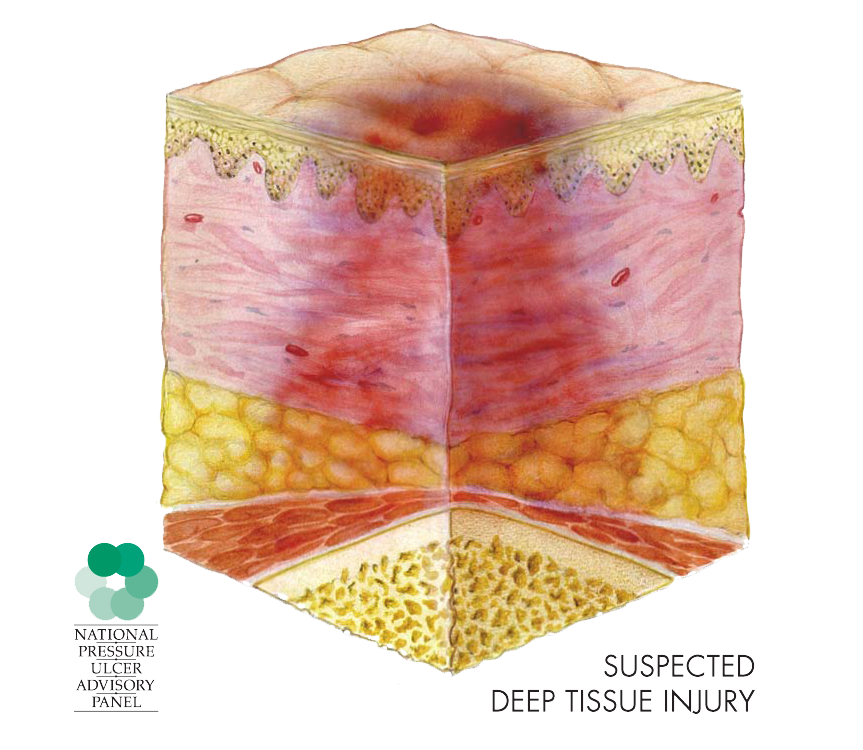
\includegraphics[width=\textwidth]{assets/npuap/suspectedDTI.png}
						\caption{\tiny \copyright\ National Pressure Ulcer Advisory Panel, used with permission.}
					\end{figure}
			\end{columns}
		\end{frame}

		\note{First off, the problem that this work is trying to deal with is that of deep tissue injuries, or DTI for short. DTI are wounds that generally form when a region of tissue is placed under excessive loading for extended periods of time, and as such are common injuries for people with spinal cord injuries and the elderly. These injuries are related to pressure ulcers, (or ``bedsores''), however they differ in that they form deep in the tissue at boney prominences and work their way to the surface of the skin. This attribute is what makes them extremely hard to detect, as once they burst through to the surface of the skin it is generally ``too late'' to treat the injury and it must instead be managed. All of this of course places a tremendous burden not only on the patients who suffer from these injuries but on the health care system as well.}

		\begin{frame}
			\frametitle{Current DTI Detection}
			\begin{itemize}
				\item Clinical settings: \alert{risk assessment scales}
				\begin{itemize}
					\item Norton, Braden, and Risk Assessment Pressure Sore scales
					\item No actual detection, only risk assessment
				\end{itemize}
				\item Research settings: \alert{T$_2^*$-weighted MRI}
				\begin{itemize}
					\item Not feasible clinically
				\end{itemize}
				\item New research:
				\begin{itemize}
					\item B-mode imaging (Aoi et al. \cite{aoi08})
					\item Blood / urine markers (Mahksous et al. \cite{mahksous10})
					\item \alert{Ultrasound elastography} (Deprez et al. \cite{deprez11})
				\end{itemize}
			\end{itemize}
		\end{frame}

		\note{One key method of improving DTI-suffering patient outcomes would be to implement a clinical system capable of detecting formative DTI when they are small and still easily reversible. Unfortunately, the current clinical detection standard is not really detection at all, but a series of relatively subjective ``risk assessment scales'' which provide risk estimates of injury formation, but do nothing to actually detect or monitor forming injuries. In research settings, T-2-star weighted MRI has been used to detect DTI formation, however this technique is largely not clinically relevant due to the costs associated with MRI.

		Recent research has instead turned to ultrasound for clinical DTI detection due to it's ease-of-use and relative low cost. While some researchers have had marginal success using classical b-mode imaging to detect DTI, the imaging results require a high degree of interpretation and have not been widely replicated. Biomarkers released during the breakdown of muscle tissue are being investigated as a quick and inexpensive method of determining whether an injury exists or not, however these markers suffer from a lack of localization and monitoring capability. Finally, ultrasound elastography has been presented as the most promising means of detecting and monitoring DTI due to it's ability to localize injuries at depth}

		\begin{frame}
			\frametitle{Ultrasound Elastography}
			\begin{itemize}
				\item Mechanical \alert{stiffness changes} with injury formation and progression
			\end{itemize}
			\begin{center}
				\begin{figure}
					\begin{tikzpicture}[x=0.75\textwidth,y=0.25\textwidth]
						% basal stiffness
						\draw[ultra thick, dashed]
						(0, 0.3) -- (1, 0.3);

						% stiffness curve
						\draw[ultra thick, draw=ExecusharesBlue] plot[smooth, tension=1] (0, 0.3) .. controls(0.15, 0.3) and (0.15, 1) .. (0.3, 1);
						\draw[ultra thick, ->, draw=ExecusharesBlue] plot[smooth, tension=1] (0.3, 1) .. controls(0.45, 1) and (0.45, 0.1) .. (1, 0.1);

						% axes
						\draw[ultra thick, <->, draw=black] (0, 1) -- (0, 0) -- (1, 0);

						% time tick
						\draw (0.3, -0.05) -- (0.3, 0.05);

						\node[below] at (0.15, 0) {Hours};
						\node[below] at (0.6, 0) {Days};
						\node[rotate=90] at (-0.05, 0.75) {Stiffness};
						\node[left] at (0, 0.3) {\scriptsize Basal Stiffness};
						\node at (0.3125, 0.6) {\footnotesize Local Rigor Mortis};
						\node at (0.9, 0.2) {\footnotesize Decomposition};
						\node at (0.9, -0.1) {Time};
					\end{tikzpicture}
					\caption{Adapted from Gefen \cite{gefen09}, used with permission}
				\end{figure}
			\end{center}
			\vspace{-0.5cm}
			\begin{itemize}
				\item Ultrasound elastography is a technology which measures tissue \alert{stiffness}
			\end{itemize}
		\end{frame}

		\note{Ultrasound elastography is able to distinguish DTI based on one key fact: as deep tissue injuries form and progress, the tissue undergoes substantial mechanical stiffness changes. Since ultrasound elastography is able to image localized differences in tissue stiffness, it follows that ultrasound elastography can detect and monitor the stiffness changes associated with DTI.}

		\begin{frame}
			\frametitle{Literature Review}
			\begin{center}
				\vspace{1cm}
				\begin{tabular}{r|c|cccc|cccc|cc}
					& \rotHead{DTI} & \rotHead{B-Mode US} & \rotHead{QS USE} & \rotHead{ARFI} & \rotHead{Shear} & \rotHead{FE Models} & \rotHead{Gel Phantoms} & \rotHead{Animals} & \rotHead{Humans} & \rotHead{Characterized} & \rotHead{Clinical} \\
					\hline
					PU Risk scales & \xmark & --- & --- & --- & --- & \xmark & \xmark & \xmark & \cmark & \cmark & \cmark \\
					T$_2^*$ MRI & \cmark & --- & --- & --- & --- & \cmark & \cmark & \cmark& \cmark & \xmark & \xmark \\
					\hline
					Aoi et al. \cite{aoi08} & \cmark & \cmark & \xmark & \xmark & \xmark & \xmark & \xmark & \xmark & \cmark & \xmark & \color{ExecusharesBlue}\textbf{?} \\
					Mahksous et al. \cite{mahksous10} & \cmark & --- & --- & --- & --- & --- & --- & \cmark & \xmark & \xmark & \cmark \\
					Deprez et al. \cite{deprez11} & \cmark & \xmark & \cmark & \xmark & \xmark & \cmark & \cmark & \cmark & \xmark & \xmark & \cmark \\
					\hline
					This work & \cmark & \xmark & \cmark & \cmark & \cmark & \cmark & \cmark & \color{ExecusharesBlue}\textbf{?} & \color{ExecusharesBlue}\textbf{?} & \cmark & \cmark \\
				\end{tabular}
			\end{center}
			\begin{itemize}
				\item The \alert{purpose} of this research was to gain understanding of and characterize the use of ultrasound elastography toward DTI detection
			\end{itemize}
		\end{frame}

		\note{The purpose of this work then was to characterize the use of ultrasound elastography toward the detection of DTI such that it may eventually be used clinically. This work is different from other DTI detection techniques largely by it's inclusion of ARFI imaging and shear wave speed quantification as well as numerical characterizations of a wide array of parameters on the detection sensitivity of the technique, and you can see how this work compares to other techniques and previous work here.}

	\setbeamertemplate{section page}
	{
		\begin{tikzpicture}
			% set up the entire slide as the canvas
			\useasboundingbox (0,0) rectangle(\the\paperwidth,\the\paperheight);
			\fill[color=ExecusharesWhite] (-1cm, 1cm) rectangle(11.8cm, 9.8cm);
			\fill[color=ExecusharesRed] (-1cm, 3.9cm) rectangle(11.8cm, 5.9cm);
			\node[text width=11.8cm,align=center] at (5.4cm, 4.9cm) {\color{ExecusharesWhite}\Huge\textbf{\insertsection *}};
			\node[text width=11.8cm,align=center,anchor=north] at (5.4cm, 3.9cm) {\color{ExecusharesGrey} \small * Accepted for publication as: K. Hamaluik, W. Moussa, and M. Ferguson-Pell, ``Numerical Characterization of Quasi-Static Ultrasound Elastography for the Detection of Deep Tissue Injuries.'' \emph{IEEE Transactions on Medical Imaging} };
		\end{tikzpicture}
	}
	\section[QS USE]{Quasi-Static Ultrasound Elastography}
		\setbeamertemplate{section page}
		{
			\begin{tikzpicture}
				% set up the entire slide as the canvas
				\useasboundingbox (0,0) rectangle(\the\paperwidth,\the\paperheight);
				\fill[color=ExecusharesWhite] (-1cm, 1cm) rectangle(11.8cm, 9.8cm);
				\fill[color=ExecusharesRed] (-1cm, 3.9cm) rectangle(11.8cm, 5.9cm);
				\node[text width=11.8cm,align=center] at (5.4cm, 4.9cm) {\color{ExecusharesWhite}\Huge\textbf{\insertsection}};
			\end{tikzpicture}
		}

		\begin{frame}
			\frametitle{Introduction}
			\vspace{0.5cm}
			\begin{itemize}
				\item Earliest form of ultrasound elastography
				\item Apply manual pressure to tissue
				\begin{itemize}
					\item Measure localized deformation of tissue
				\end{itemize}
				\item Magnitude of deformation related to stiffness
				\begin{itemize}
					\item $\downarrow$ deformation $\approx$ $\uparrow$ stiffness $\approx$ $\uparrow$ damage magnitude
				\end{itemize}
			\end{itemize}

			\vspace{0.5cm}
			\begin{columns}[b]
				\column{0.5\textwidth}
					\begin{tikzpicture}[x=\textwidth,y=0.4\textwidth]
						\draw[thick, draw=ExecusharesBlack, fill=ExecusharesWhite]
						(0, 0) -- (1, 0) -- (1, 1) -- (0, 1) -- cycle;
						\draw[dashed, thick, draw=ExecusharesBlack, fill=none]
						(0.15, 0.1) -- (0.85, 0.1) -- (0.85, 1) -- (0.15, 1) -- cycle;
						\draw[thick, draw=ExecusharesBlack, fill=ExecusharesRed]
						(0.15, 1) -- (0.85, 1) -- (0.85, 1.25) -- (0.15, 1.25) -- cycle;
						\draw[ultra thick, draw=ExecusharesBlue, fill=none]
						(0.55, 0.45) -- (0.65, 0.45) -- (0.65, 0.75) -- (0.55, 0.75) -- cycle;
						\tikzset{text=ExecusharesBlue}
						\node at (0.6, 0.6) {$R_1$};
						\tikzset{text=ExecusharesBlack}
						\node at (0.5, 1.125) {US Probe};
						\tikzset{text=ExecusharesBlack}
						\node at (0.5, 0.25) {Field of View};
						\tikzset{text=ExecusharesBlack}
						\node at (0.5, -0.15) {Pre-compression image};
					\end{tikzpicture}

				\column{0.5\textwidth}
					\begin{tikzpicture}[x=\textwidth,y=0.4\textwidth]
						\draw[thick, draw=ExecusharesBlack, fill=ExecusharesWhite]
						(0, 0) -- (1, 0) -- (1, 0.8) -- (0, 0.8) -- cycle;
						\draw[dashed, thick, draw=ExecusharesBlack, fill=none]
						(0.15, 0.1) -- (0.85, 0.1) -- (0.85, 0.8) -- (0.15, 0.8) -- cycle;
						\draw[thick, draw=ExecusharesBlack, fill=ExecusharesRed]
						(0.15, 0.8) -- (0.85, 0.8) -- (0.85, 1.05) -- (0.15, 1.05) -- cycle;
						\draw[thick, draw=ExecusharesBlack, fill=ExecusharesBlue]
						(0.5, 1.1) -- (0.6, 1.2) -- (0.55, 1.2) -- (0.55, 1.25) -- (0.45, 1.25) -- (0.45, 1.2) -- (0.4, 1.2) -- cycle;
						\draw[ultra thick, draw=ExecusharesBlue, fill=none]
						(0.65, 0.45) -- (0.75, 0.45) -- (0.75, 0.65) -- (0.65, 0.65) -- cycle;
						\tikzset{text=ExecusharesBlue}
						\node at (0.7, 0.55) {$R_2$};
						\draw[ultra thick, ->, draw=ExecusharesBlue, fill=ExecusharesBlue]
						(0.55, 0.4) -- (0.65, 0.45);
						\tikzset{text=ExecusharesBlack}
						\node at (0.5, 0.925) {US Probe};
						\tikzset{text=ExecusharesBlack}
						\node at (0.5, 0.25) {Field of View};
						\node at (0.5, -0.15) {Post-compression image};
					\end{tikzpicture}
			\end{columns}
		\end{frame}

		\note{The first imaging modality I investigated was ``quasi-static ultrasound elastography'', which involves the manual manipulation of soft tissues in order to estimate deformation gradients and subsequently localized tissue strains. By comparing localized tissue strains throughout the domain, the stiffness ratio of lesions may be estimated.}

		\begin{frame}
			\frametitle{Tracking Localized Deformation}
			\begin{columns}[c]
				\column{0.6\textwidth}
					\begin{itemize}
						\item ``Noise'' isn't actually noise
						\begin{itemize}
							\item Scattering centres anchored in tissue
						\end{itemize}
						\item Track motion of scattering centres between pre/post compression
						\begin{itemize}
							\item Under assumptions of motion (Brusseau et al. \cite{brusseau08})
						\end{itemize}
					\end{itemize}

				\column{0.4\textwidth}
					\begin{figure}
						\centering
						\subfloat{%
							\begin{tikzpicture}
								\node at (0, 0){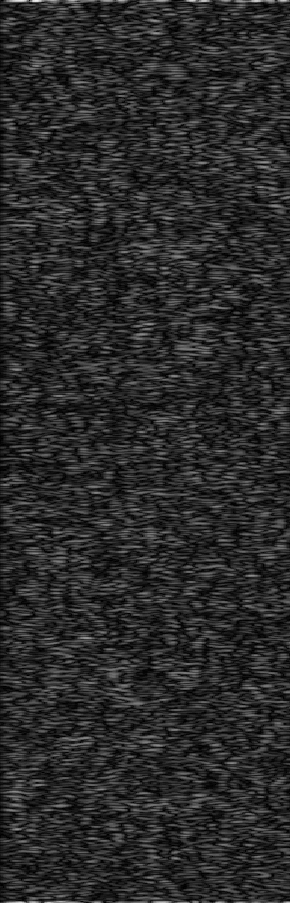
\includegraphics[height=6cm]{../latex/assets/quasistatic/images/bModeA.png}};
								\draw[draw=ExecusharesBlue] (0, -1.7cm) ellipse (0.25cm and 0.125cm);
								\draw[draw=ExecusharesRed] (0.75cm, 1.9cm) circle(0.2cm);
							\end{tikzpicture}
						}
						~
						\subfloat{%
							\begin{tikzpicture}
								\node at (0, 0){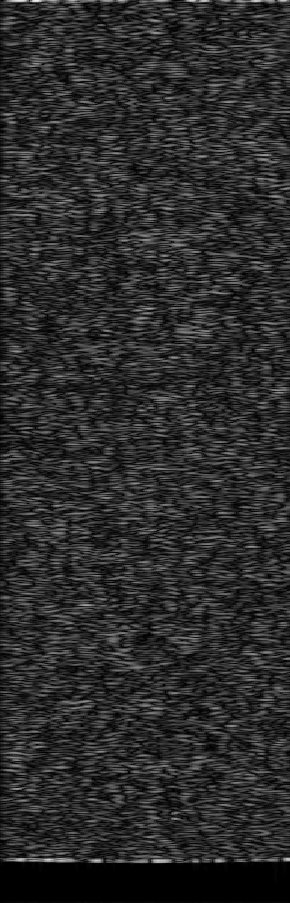
\includegraphics[height=6cm]{../latex/assets/quasistatic/images/bModeB.png}};
								\draw[draw=ExecusharesBlue] (0, -1.45cm) ellipse (0.25cm and 0.125cm);
								\draw[draw=ExecusharesRed] (0.75cm, 1.95cm) circle(0.2cm);
							\end{tikzpicture}
						}
						\caption{Pre- and Post- Compression B-Mode Images of DTI}
					\end{figure}
			\end{columns}
		\end{frame}

		\note{In order to obtain the localized strains in the soft tissue domain, this technique calculates the motion of scattering centres throughout the tissue. If one set of scattering centres deforms less than its surroundings, that region of tissue may be considered to be relatively stiff. In order to generate this simulated b-mode ultrasound images, I utilized the convolution of a randomly seeded domain with the point-spread-function of the transducer. Deformation was applied to this tissue using a static finite-element model of tissue deformation in response the externally applied loading.}

		\begin{frame}
			\frametitle{Investigated Models}
			\begin{figure}
				\centering
				\subfloat{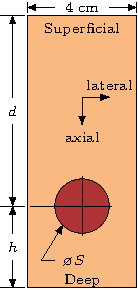
\includegraphics[width=0.84375in]{../latex/assets/quasistatic/drawings/schematic_single-crop.pdf}}
				~
				\subfloat{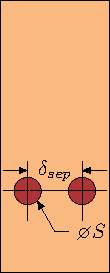
\includegraphics[width=0.68612625in]{../latex/assets/quasistatic/drawings/schematic_colocated-crop.pdf}}
				~
				\subfloat{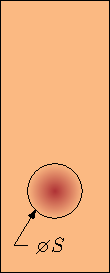
\includegraphics[width=0.68612625in]{../latex/assets/quasistatic/drawings/schematic_blur-crop.pdf}}
				~
				\subfloat{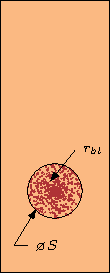
\includegraphics[width=0.68612625in]{../latex/assets/quasistatic/drawings/schematic_blob-crop.pdf}}
				~
				\subfloat{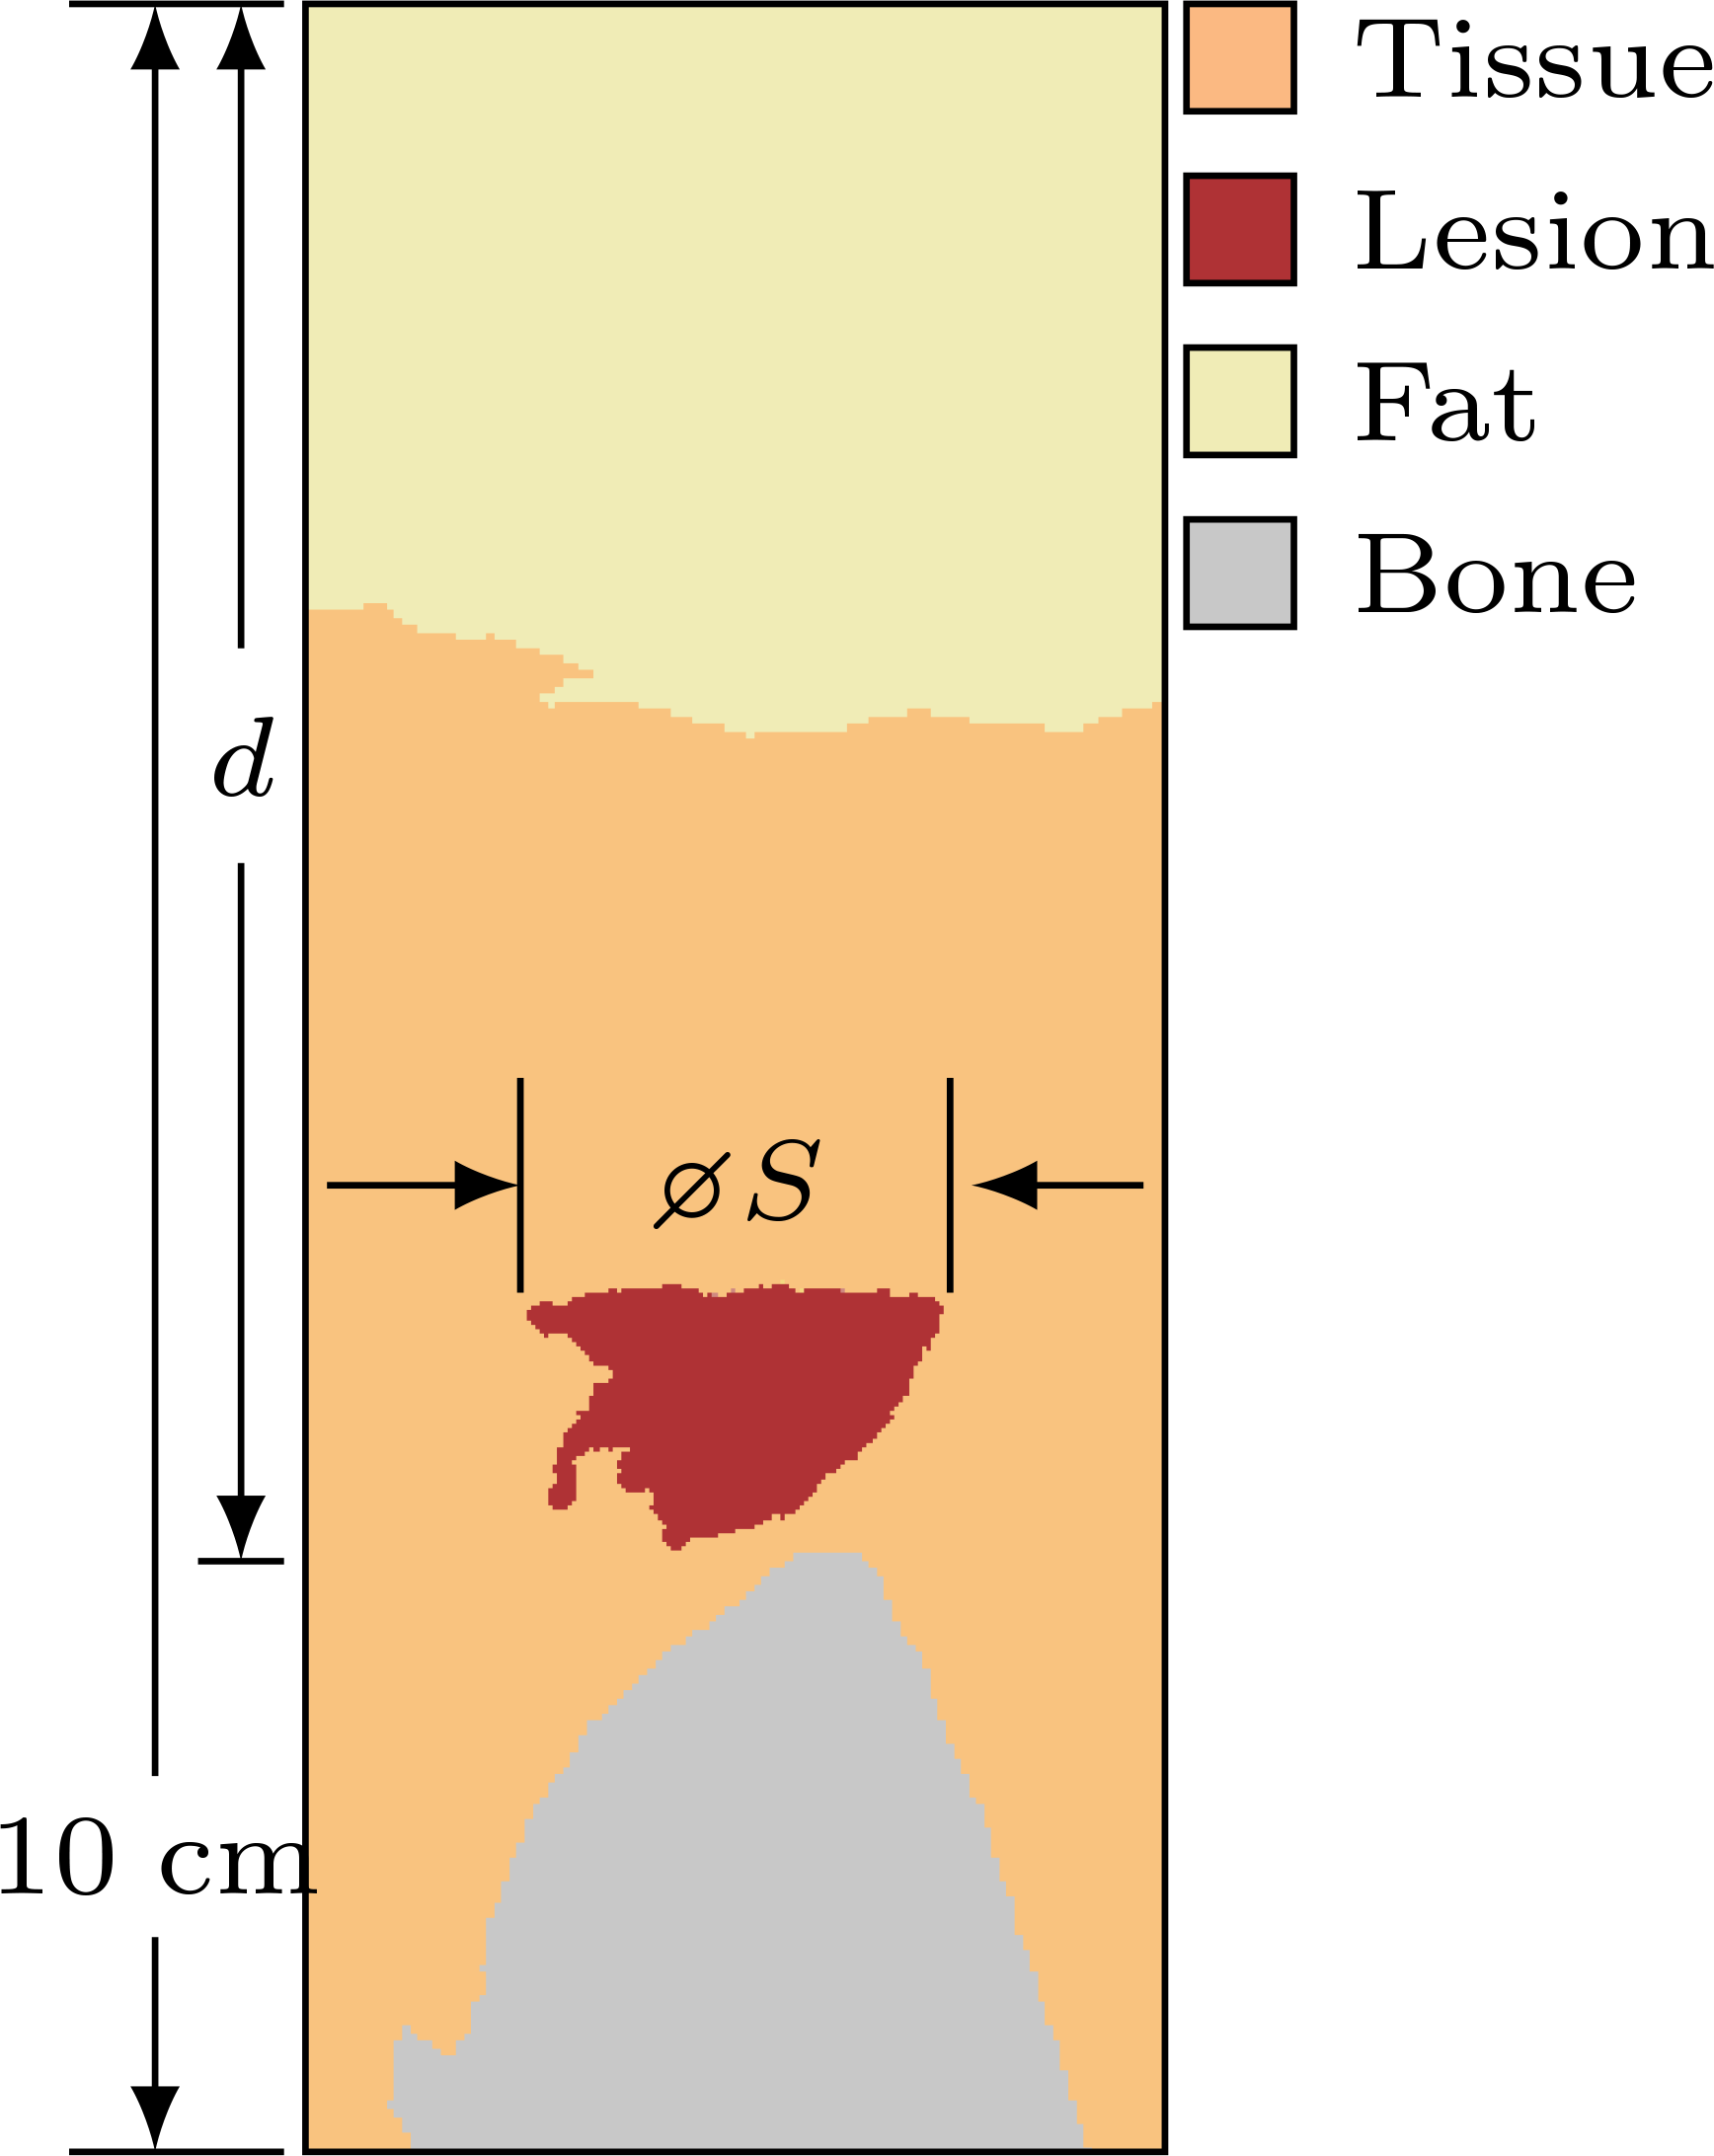
\includegraphics[width=1.34443125in]{../latex/assets/quasistatic/drawings/schematic_human-crop.png}}
			\end{figure}
		\end{frame}

		\note{In an effort to investigate a wide range of parameters, the various models you see here were evaluated, ranging from a simple ``spherical'' lesion to investigate overarching parameters such as lesion size and depth to a complicated geometry obtained from the combination of Visible Human data and and MRI-acquired image of a DTI in a pig model. A parametric study on all of the parameters you see here was carried out in order to determine how each variable affects the detection sensitivity of quasi-static elastography.}

		\begin{frame}
			\frametitle{Sample Resultant Elastogram}
			\vspace{-0.5cm}
			\begin{figure}
				\centering
				\subfloat{%
					\begin{tikzpicture}
						\begin{axis}[height=7cm, enlargelimits=false, unit vector ratio*=1 1 1, axis on top, xlabel={$x$ (\si{\cm})}, ylabel={Depth, $d$ (\si{\cm})}, xtick={-2,0,2}, y dir=reverse, draw=ExecusharesBlack, text=ExecusharesBlack, fill=ExecusharesBlack]
							\addplot graphics[xmin=-2,xmax=2,ymin=0,ymax=12.5]{../latex/assets/quasistatic/images/bModeA.png};
						\end{axis}
					\end{tikzpicture}
				}
				~
				\subfloat{%
					\begin{tikzpicture}
						\useasboundingbox (0,0) rectangle(0.1in,3in);
						\node at(0.05in, 1.5in){$+$};
					\end{tikzpicture}
				}
				~
				\subfloat{%
					\begin{tikzpicture}
						\begin{axis}[height=7cm, enlargelimits=false, unit vector ratio*=1 1 1, axis on top, xlabel={$x$ (\si{\cm})}, xtick={-2,0,2}, yticklabels={,,}, draw=ExecusharesBlack, text=ExecusharesBlack, fill=ExecusharesBlack]
							\addplot graphics[xmin=-2,xmax=2,ymin=0,ymax=12.5]{../latex/assets/quasistatic/images/bModeB.png};
						\end{axis}
					\end{tikzpicture}
				}
				~
				\subfloat{%
					\begin{tikzpicture}
						\useasboundingbox (0,0) rectangle(0.25in,3in);
						\draw[->] (0in, 1.5in) -- (0.3in, 1.5in);
					\end{tikzpicture}
				}
				~
				\subfloat{%
					\begin{tikzpicture}
						\begin{axis}[height=7cm, enlargelimits=false, unit vector ratio*=1 1 1, axis on top, xlabel={$x$ (\si{\cm})}, xtick={-2,0,2}, yticklabels={,,}, draw=ExecusharesBlack, text=ExecusharesBlack, fill=ExecusharesBlack, colormap name={YlOrRd}, colorbar, point meta min=0, point meta max=7, colorbar style={yticklabel={\pgfmathprintnumber{\tick}\,\percent},at={(1.05,0)}, width=0.02\textwidth, ylabel={Compressive Strain}, anchor=south west, draw=ExecusharesBlack, text=ExecusharesBlack, fill=ExecusharesBlack}]
							\addplot graphics[xmin=-2,xmax=2,ymin=0,ymax=12.5]{../latex/assets/quasistatic/elastograms/e040_colour.png};
						\end{axis}
					\end{tikzpicture}
				}
			\end{figure}
		\end{frame}

		\note{And here we see a sample result from these simulations, combining the pre and post compression b-mode images (in which no lesion is visible), and calculating the strain field which very clearly depicts a large stiff lesion in this lower portion of the image.}

		\begin{frame}
			\frametitle{Sample Quasi-Static Results}
			\begin{figure}
				\centering
				\subfloat{%
					\characterizationPic{%
						\characterizationPlots{strainRatio}%
							{quasistatic/data/circular_size_05.dat}%
							{quasistatic/data/circular_size_10.dat}%
							{quasistatic/data/circular_size_20.dat}%
							{quasistatic/data/circular_size_25.dat}%
					}{%
						\characterizationLegend{Lesion Diameter}{\diameter S}%
							{\SI{0.5}{\cm}}%
							{\SI{1.0}{\cm}}%
							{\SI{2.0}{\cm}}%
							{\SI{2.5}{\cm}}%
					}{spherical_size}{0,2.5}{north west}{ymin=0.5,ymax=2.5}
				}
				\vspace{-0.25cm}
				\subfloat{%
					\characterizationPic{%
						\characterizationPlots{strainRatio}%
							{quasistatic/data/circular_depth_035.dat}%
							{quasistatic/data/circular_depth_065.dat}%
							{quasistatic/data/circular_depth_085.dat}%
							{quasistatic/data/circular_depth_100.dat}%
					}{%
						\characterizationLegend{Lesion Depth}{d}%
							{\SI{3.5}{\cm}}%
							{\SI{6.5}{\cm}}%
							{\SI{8.5}{\cm}}%
							{\SI{10.0}{\cm}}%
					}{spherical_depth}{0,2.5}{north west}{ymin=0.5,ymax=2.5}
				}
			\end{figure}
		\end{frame}

		\begin{frame}
			\frametitle{Sample Quasi-Static Results}
			\begin{figure}
				\centering
				\subfloat{%
				\characterizationPic{%
						\characterizationPlots{strainRatio}%
							{quasistatic/data/circular_frequency_2.dat}%
							{quasistatic/data/circular_frequency_4.dat}%
							{quasistatic/data/circular_frequency_8.dat}%
					}{%
						\characterizationLegend{Probing Frequency}{f}%
							{\SI{2}{\MHz}}%
							{\SI{4}{\MHz}}%
							{\SI{8}{\MHz}}%
					}{spherical_frequency}{0,2.25}{north west}{ymin=0.5,ymax=2.25}
				}
				\vspace{-0.25cm}
				\subfloat{%
					\characterizationPic{%
						\characterizationPlots{strainRatio}%
							{quasistatic/data/circular_strain_025.dat}%
							{quasistatic/data/circular_strain_050.dat}%
							{quasistatic/data/circular_strain_100.dat}%
					}{%
						\characterizationLegend{Applied Strain}{\varepsilon_{app}}%
							{\SI{2.5}{\percent}}%
							{\SI{5.0}{\percent}}%
							{\SI{10.0}{\percent}}%
					}{spherical_strain}{0,2.25}{north west}{ymin=0.5,ymax=2.25}
				}
			\end{figure}
		\end{frame}

		\note{By then comparing the strain ratio between lesionous regions and the surrounding ``healthy'' tissue, }

		\begin{frame}
			\frametitle{Quasi-Static USE Outcomes}
			\begin{itemize}
				\item QS USE \alert{is} capable of DTI detection
				\item Detection sensitivity less than desirable
				\item Manual palpation is not ideal
				\begin{itemize}
					\item Suggest \alert{ARFI imaging} for machine-induced tissue deformation instead
				\end{itemize}
				\item Small lesions almost undetectable
				\item Use $\leq$ \SI{5}{\percent} applied strain
				\item Depth, interrogation frequency don't affect detection ability
			\end{itemize}
		\end{frame}

	\section[ARFI]{Acoustic Radiation Force Impulse Imaging}
		\begin{frame}
			\frametitle{Introduction}
			\begin{itemize}
				\item QS USE has low detection sensitivity, manual palpation is difficult and unreliable
				\item \alert{ARFI} imaging works on the same principles as QS USE
				\begin{itemize}
					\item But uses \alert{transducer-generated} force to displace tissue
				\end{itemize}
				\item $\uparrow$ repeatability, $\uparrow$ inter-operator reliability
				\item By imparting acoustic energy to the tissue, body force is generated:

					\begin{equation*}
						\left|\vec{F}\right| = \frac{2\alpha I}{c}
					\end{equation*}
			\end{itemize}
		\end{frame}

		\begin{frame}
			\frametitle{How ARFI Imaging Works}
			\begin{columns}[t]
				\column{0.5\textwidth}
					\begin{itemize}
						\item Normal ultrasound is only a couple periods long ($\approx \SI{2}{\ms}$)
					\end{itemize}

					\begin{center}
						\begin{tikzpicture}
							\draw[draw=ExecusharesBlack, fill=ExecusharesRed] (0, 3) -- (0, 3.2) -- (0.5, 3.4) -- (0.5, 3.6) -- (1.5, 3.6) -- (1.5, 3.4) -- (2, 3.2) -- (2, 3);
							\draw[draw=ExecusharesBlack, fill=white] (0, 0) rectangle(2, 3);
							\draw[domain=0:1,samples=50,variable=\y,draw=ExecusharesBlack] plot ({cos(320*pi*\y+180)*gauss(0.5,0.25,\y)*0.25+1},{\y+1.4});
							\draw[draw=ExecusharesBlack,->] (1, 1.25) -- (1, 0.75);
						\end{tikzpicture}
					\end{center}

				\column{0.5\textwidth}
					\begin{itemize}
						\item ARFI imaging uses continuous beams ($\approx \SI{100}{\ms}$)
					\end{itemize}

					\begin{center}
						\begin{tikzpicture}
							\draw[draw=ExecusharesBlack, fill=ExecusharesRed] (0, 3) -- (0, 3.2) -- (0.5, 3.4) -- (0.5, 3.6) -- (1.5, 3.6) -- (1.5, 3.4) -- (2, 3.2) -- (2, 3);
							\draw[draw=ExecusharesBlack, fill=white] (0, 0) rectangle(2, 3);
							\draw[domain=0:3, samples=150, variable=\y,ExecusharesBlack] plot ({cos(320*pi*\y+180)*0.25+1},{\y});
							\draw[draw=ExecusharesBlack,->] (0.5, 1.75) -- (0.5, 1.25);
							\draw[draw=ExecusharesBlack,->] (1.5, 1.75) -- (1.5, 1.25);
						\end{tikzpicture}
					\end{center}
			\end{columns}

			\begin{itemize}
				\item Acoustic energy is absorbed by tissue and causes deformation
			\end{itemize}
		\end{frame}

		\begin{frame}
			\frametitle{Simulating ARFI Loads}
			\vspace{0.75cm}
			\begin{itemize}
				\item Use k-space pseudo-spectral method to solve the wave equation
				\begin{itemize}
					\item k-Wave MATLAB\textsuperscript{\textregistered}\ toolbox
				\end{itemize}
			\end{itemize}
			\vspace{-0.75cm}
			\hspace{1cm}
			\begin{center}
				\begin{figure}
					\centering
					\subfloat{%
						\begin{tikzpicture}
							\begin{axis}
								[
								font=\tiny,
								scale only axis,
								enlargelimits=false,
								unit vector ratio*=1 1 1,
								width=0.5\textwidth,
								y dir=reverse,
								xlabel={X-Coordinate, $x$ (\si{\cm})},
								ylabel={Depth, $d$ (\si{\cm})},
								axis on top]
									\addplot graphics[xmin=-2,xmax=2,ymin=0,ymax=10]{../latex/assets/shear/data/Fx158.png};
							\end{axis}
							\node[anchor=south] at(0.9, 4.75) {\scriptsize Lateral Force};
						\end{tikzpicture}
					}
					\subfloat{%
						\begin{tikzpicture}
							\begin{axis}
								[
								font=\tiny,
								scale only axis,
								enlargelimits=false,
								unit vector ratio*=1 1 1,
								width=0.5\textwidth,
								y dir=reverse,
								yticklabels={,,},
								xlabel={X-Coordinate, $x$ (\si{\cm})},
								axis on top,
								colormap name={RdBu},
								colorbar, point meta min=-175, point meta max=175, colorbar style={at={(1.05,0)}, font=\tiny, ytick={-175,-100,0,100,175}, anchor=south west, width=0.03\textwidth, ylabel={Acoustic Radiation Force, $F_{ARFI}$ (\si{\kN\per\metre\cubed})},
								draw=black, text=black, fill=black}]
									\addplot graphics[xmin=-2,xmax=2,ymin=0,ymax=10]{../latex/assets/shear/data/Fy158.png};
							\end{axis}
							\node[anchor=south] at(0.9, 4.75) {\scriptsize Axial Force};
						\end{tikzpicture}
					}
				\end{figure}
			\end{center}
		\end{frame}

		\begin{frame}
			\frametitle{Sample ARFI Results}
			\vspace{0.25cm}
			\begin{figure}
				\centering
				\subfloat{%
					\begin{tikzpicture}
						\begin{axis}[
							scale only axis,
							height=0.25\textwidth,%
							width=0.6\textwidth,%
							font=\tiny,
							axis background/.style={fill=white},
							xlabel={Focal Depth, $d_{f}$ (\si{\cm})},
							ylabel style={align=center},
							ylabel={Maximum Induced Tissue \\ Displacement, $\left|v\right|_{max}$ (\si{\charmu\metre})},
							grid=major,
							legend entries={\textbf{Interrogation}, \textbf{Frequency}, $f = \SI{1}{\MHz}$, $f = \SI{2}{\MHz}$, $f = \SI{4}{\MHz}$, $f = \SI{6}{\MHz}$},
							legend style={legend cell align=left, legend pos=outer north east,font=\tiny,nodes={right}},
							clip=true,
							cycle list name=ColourPlotCycle,
							draw=black, text=black, fill=black]
							\addlegendimage{empty legend};
							\addlegendimage{empty legend};
							\addplot table[x expr=\thisrow{depth}*100, y expr=\thisrow{maxDisp}*1e6] {../latex/assets/arfi/data/depth_maxDisp_freq1.dat};
							\addplot table[x expr=\thisrow{depth}*100, y expr=\thisrow{maxDisp}*1e6] {../latex/assets/arfi/data/depth_maxDisp_freq2.dat};
							\addplot table[x expr=\thisrow{depth}*100, y expr=\thisrow{maxDisp}*1e6] {../latex/assets/arfi/data/depth_maxDisp_freq4.dat};
							\addplot table[x expr=\thisrow{depth}*100, y expr=\thisrow{maxDisp}*1e6] {../latex/assets/arfi/data/depth_maxDisp_freq6.dat};
							\node [anchor=north east](c) at (axis cs:9.5,4.2) {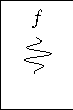
\includegraphics[width=0.5cm]{../latex/assets/insets/nolesion_frequency.pdf}};
						\end{axis}
					\end{tikzpicture}
				}
				\vspace{-0.25cm}
				\subfloat{%
					\begin{tikzpicture}
						\begin{axis}[
							scale only axis,
							height=0.25\textwidth,%
							width=0.6\textwidth,%
							font=\tiny,
							axis background/.style={fill=white},
							xlabel={Focal Depth, $d_{f}$ (\si{\cm})},
							ylabel style={align=center},
							ylabel={Spatial-Peak Pulse-Average \\ Intensity, $I_{SPPA}$ (\si{\watt\per\cm\squared})},
							grid=major,
							legend entries={\textbf{Interrogation}, \textbf{Frequency}, $f = \SI{1}{\MHz}$, $f = \SI{2}{\MHz}$, $f = \SI{4}{\MHz}$, $f = \SI{6}{\MHz}$, Acceptable limit},
							legend style={legend cell align=left, legend pos=outer north east,font=\tiny,nodes={right}},
							clip=true,
							xmin=0,xmax=10,ymin=0,ymax=2250,
							cycle list name=ColourPlotCycle,
							draw=black, text=black, fill=black]
							\addlegendimage{empty legend};
							\addlegendimage{empty legend};
							\addplot table {../latex/assets/arfi/data/depth_isppa_freq1.dat};
							\addplot table {../latex/assets/arfi/data/depth_isppa_freq2.dat};
							\addplot table {../latex/assets/arfi/data/depth_isppa_freq4.dat};
							\addplot table {../latex/assets/arfi/data/depth_isppa_freq6.dat};
							\addplot[mark=none,dashed,thick,draw=ExecusharesGrey] plot coordinates {(0, 933) (10, 933)};
							\draw (axis cs:7,933) node[below]{\color{ExecusharesGrey} Acceptable};
							\draw (axis cs:7,933) node[above]{\color{ExecusharesGrey} Unacceptable};
						\end{axis}
					\end{tikzpicture}
				}
			\end{figure}
		\end{frame}

		\begin{frame}
			\frametitle{Sample ARFI Results}
			\vspace{0.25cm}
			\begin{figure}
				\centering
				\subfloat{%
					\characterizationPic{%
						\characterizationPlots{esr}%
							{arfi/data/arfi_radius_r025.dat}%
							{arfi/data/arfi_radius_r050.dat}%
							{arfi/data/arfi_radius_r100.dat}%
							{arfi/data/arfi_radius_r125.dat}%
					}{%
						\characterizationLegend{Lesion Radius}{r_{lesion}}%
							{\SI{2.5}{\mm}}%
							{\SI{5.0}{\mm}}%
							{\SI{10.0}{\mm}}%
							{\SI{12.5}{\mm}}%
					}{spherical_radius}{0, 2.5}{north west}{ymin=0.5,ymax=2.5}
				}
				\vspace{-0.25cm}
				\subfloat{%
					\characterizationPic{%
						\characterizationPlots{esr}%
							{arfi/data/arfi_maxDisp_depth_d2.dat}%
							{arfi/data/arfi_maxDisp_depth_d4.dat}%
							{arfi/data/arfi_maxDisp_depth_d6.dat}%
							{arfi/data/arfi_maxDisp_depth_d8.dat}%
					}{%
						\characterizationLegend{Lesion Depth}{d}%
							{\SI{2}{\cm}}%
							{\SI{4}{\cm}}%
							{\SI{6}{\cm}}%
							{\SI{8}{\cm}}%
					}{spherical_depth}{0,2.25}{north west}{ymin=0.5,ymax=2.25}
				}
			\end{figure}
		\end{frame}

		\begin{frame}
			\frametitle{ARFI Imaging Outcomes}
			\begin{itemize}
				\item ARFI more reliable than QS USE
				\begin{itemize}
					\item Computer-controlled deformation force
				\end{itemize}
				\item Safety implications
				\begin{itemize}
					\item High intensity acoustic waves can damage tissue
					\item Difficult to get deep penetration without damage
				\end{itemize}
				\item No effect on detection sensitivity of lesion size for radii $\geq$ \SI{2.5}{\mm}
				\item Lesion depth only a factor in generating radiation force
				\begin{itemize}
					\item Soft tissue absorption makes deep penetration difficult
				\end{itemize}
				\item Better at interrogating complicated geometry than QS USE
			\end{itemize}
		\end{frame}

	\section[Shear]{Shear Wave Speed Quantification}
		\begin{frame}
			\frametitle{Introduction}
			\begin{itemize}
				\item QS USE and ARFI only provide \alert{qualitative} measures of stiffness
				\item Measuring shear wave speed allows quantifiable calculation of stiffness
				\begin{itemize}
					\item Can be used to accurately track over time and give absolute references
				\end{itemize}
				\item Uses ARFI pulses to generate shear waves in tissue
				\begin{itemize}
					\item Measure shear wave speed $\rightarrow$ calculate stiffness:
				\end{itemize}
			\end{itemize}
			\begin{equation*}
				\mu = c_T^2 \rho
			\end{equation*}
		\end{frame}

		\begin{frame}
			\frametitle{Measuring Shear Wave Speed}
			\vspace{1cm}
			\begin{enumerate}
				\item<1-> Induce ARFI at desired depth
				\begin{itemize}
					\item Shear waves radiate outward, like ``ripples in a pond''
				\end{itemize}
				\item<2-> Monitor deformation along a line extending from the focal point using B-mode ultrasound
				\begin{itemize}
					\item<4-> Calculate speed of shear wave along this line
				\end{itemize}
			\end{enumerate}

			\only<1>{\vspace{-0.2cm}}
			\only<4>{\vspace{-0.49cm}}
			\begin{figure}
				\centering
				\begin{tikzpicture}
					\only<1>{\begin{axis}[
						font=\scriptsize,
						scale only axis,
						width=0.6\textwidth,
						axis background/.style={fill=white},%
						height=3cm,
						xlabel={Distance from centerline, $x$ (\si{\cm})},
						ylabel style={align=center},
						ylabel={Axial displacement, \\ $v$ (\si{\charmu\m})},
						grid=major,
						legend entries={$t = \SI{2.5}{\ms}$, $t = \SI{7.5}{\ms}$, $t = \SI{12.5}{\ms}$, $t = \SI{17.5}{\ms}$, $t = \SI{22.5}{\ms}$, $t = \SI{27.5}{\ms}$},
						legend style={legend cell align=left, legend pos=outer north east,font=\tiny},
						clip=true,
						cycle list name=SmoothColourPlotCycle,
						draw=black, text=black, fill=black,
						xmin=0, xmax=5,
						ymin=-0.75, ymax=0.5]
						\addplot table[x expr=\thisrow{x}*100, y expr=\thisrow{v}*1e6] {../latex/assets/shear/data/shear_lateral_i158_t025.dat};
						\addplot table[x expr=\thisrow{x}*100, y expr=\thisrow{v}*1e6] {../latex/assets/shear/data/shear_lateral_i158_t075.dat};
						\addplot table[x expr=\thisrow{x}*100, y expr=\thisrow{v}*1e6] {../latex/assets/shear/data/shear_lateral_i158_t125.dat};
						\addplot table[x expr=\thisrow{x}*100, y expr=\thisrow{v}*1e6] {../latex/assets/shear/data/shear_lateral_i158_t175.dat};
						\addplot table[x expr=\thisrow{x}*100, y expr=\thisrow{v}*1e6] {../latex/assets/shear/data/shear_lateral_i158_t225.dat};
						\addplot table[x expr=\thisrow{x}*100, y expr=\thisrow{v}*1e6] {../latex/assets/shear/data/shear_lateral_i158_t275.dat};
					\end{axis}}
					\only<2>{\begin{axis}[
						font=\scriptsize,
						scale only axis,
						enlargelimits=false,
						width=0.85\textwidth,
						height=3cm,
						xlabel={Time, $t$ (\si{\ms})},
						ylabel style={align=center},
						ylabel={Distance from \\ centerline, $x$ (\si{\cm})},
						axis on top]
							\addplot graphics[xmin=0,xmax=31.7,ymin=0,ymax=5]{../latex/assets/shear/data/lateralCut158.png};
					\end{axis}}
					\only<3>{\begin{axis}[
						font=\scriptsize,
						scale only axis,
						enlargelimits=false,
						width=0.85\textwidth,
						height=3cm,
						xlabel={Time, $t$ (\si{\ms})},
						ylabel style={align=center},
						ylabel={Distance from \\ centerline, $x$ (\si{\cm})},
						axis on top]
							\addplot graphics[xmin=0,xmax=31.7,ymin=0,ymax=5]{../latex/assets/shear/data/lateralCut158.png};
							\addplot[draw=black, solid, ultra thick] table[x expr=\thisrow{t}*1000, y expr=\thisrow{x}*100] {../latex/assets/shear/data/shear_lateral_i158_isoline.dat};
							\draw[ultra thick, <->, draw=black] (axis cs:15,0.75) -- (axis cs:15,1.75);
							\draw[ultra thick, draw=black, dashed] (axis cs:0,0.75) -- (axis cs:17.25,0.75);
							\draw[ultra thick, draw=black, dashed] (axis cs:0,1.75) -- (axis cs:17.25,1.75);
							\node[right] at (axis cs:15,1.25) {Lesion};
							\draw[ultra thick, ->, draw=black] (axis cs:25.65,2.75) -- (axis cs:25.65,3.7755102040816);
							\node[below] at (axis cs:25.65,2.75) {Contour line};
					\end{axis}}
					\only<4>{\begin{axis}[
						font=\scriptsize,
						scale only axis,
						width=0.85\textwidth,
						height=3cm,
						xlabel={Distance from centerline, $x$ (\si{\cm})},
						ylabel style={align=center},%
						ylabel={Shear Wave Speed, \\ $c_t$ (\si{\m\per\s})},
						grid=major,
						clip=true,
						axis background/.style={fill=white},
						draw=black, text=black, fill=black]
						\addplot[solid, ultra thick, ExecusharesBlue] table[x expr=\thisrow{x}*100] {../latex/assets/shear/data/shear_lateral_i158_shear_wave_speed.dat};

						\draw[ultra thick, ->, draw=black] (axis cs:0.25,1.8) -- (axis cs:0.75,1.8);
						\draw[ultra thick, <-, draw=black] (axis cs:1.75,1.8) -- (axis cs:2.25,1.8);
						\node[right] at (axis cs:2.25,1.8) {Lesion};
						\draw[ultra thick, draw=black, dashed] (axis cs:0.75,0) -- (axis cs:0.75,2.1);
						\draw[ultra thick, draw=black, dashed] (axis cs:1.75,0) -- (axis cs:1.75,2.1);
					\end{axis}}
				\end{tikzpicture}
			\end{figure}
		\end{frame}

		\begin{frame}
			\frametitle{Sample Shear Results}
			\begin{figure}
				\centering
				\subfloat{%
					\characterizationPic{%
						\characterizationPlots{esr}%
							{shear/data/shear_radius_r025.dat}%
							{shear/data/shear_radius_r050.dat}%
							{shear/data/shear_radius_r100.dat}%
							{shear/data/shear_radius_r125.dat}%
					}{%
						\characterizationLegend{Lesion Radius}{r_{lesion}}%
							{\SI{2.5}{\mm}}%
							{\SI{5.0}{\mm}}%
							{\SI{10.0}{\mm}}%
							{\SI{12.5}{\mm}}%
					}{spherical_radius}{0, 4.5}{north west}{ymin=0,ymax=4.5}
				}
				\vspace{-0.25cm}
				\subfloat{%
					\characterizationPic{%
						\characterizationPlots{esr}%
							{shear/data/shear_depth_o250_d2.dat}%
							{shear/data/shear_depth_o250_d4.dat}%
							{shear/data/shear_depth_o250_d6.dat}%
							{shear/data/shear_depth_o250_d8.dat}%
					}{%
						\characterizationLegend{Lesion Depth}{d}%
							{\SI{2}{\cm}}%
							{\SI{4}{\cm}}%
							{\SI{6}{\cm}}%
							{\SI{8}{\cm}}%
					}{spherical_depth}{0,4.5}{north west}{ymin=0,ymax=4.5}
				}
			\end{figure}
		\end{frame}

		\begin{frame}
			\frametitle{Sample Shear Results}
			\begin{figure}
				\centering
				\subfloat{%
					\characterizationPic{%
						\characterizationPlots{esr}%
							{shear/data/shear_doff_d4_o000.dat}%
							{shear/data/shear_doff_d4_o125.dat}%
							{shear/data/shear_doff_d4_o250.dat}%
							{shear/data/shear_doff_d4_o375.dat}%
					}{%
						\characterizationLegend{Lesion Offset}{\Delta_{off}}%
							{\SI{0.00}{\cm}}%
							{\SI{1.25}{\cm}}%
							{\SI{2.50}{\cm}}%
							{\SI{3.75}{\cm}}%
					}{offset}{0, 4.5}{north west}{ymin=0,ymax=4.5}
				}
				\vspace{-0.25cm}
				\subfloat{%
					\characterizationPic{%
						\characterizationPlots{esr}%
							{shear/data/shear_human_radius_r025.dat}%
							{shear/data/shear_human_radius_r050.dat}%
							{shear/data/shear_human_radius_r100.dat}%
							{shear/data/shear_human_radius_r125.dat}%
					}{%
						\characterizationLegend{Lesion Width}{\diameter S}%
							{\SI{5}{\mm}}%
							{\SI{10}{\mm}}%
							{\SI{20}{\mm}}%
							{\SI{25}{\mm}}%
					}{human_width}{0,4.75}{north west}{ymin=0,ymax=4.75}
				}
			\end{figure}
		\end{frame}

		\begin{frame}
			\frametitle{Shear Wave Speed Outcomes}
			\begin{itemize}
				\item More accurate than ARFI and QS USE
				\item Quantifiable
				\begin{itemize}
					\item Can monitor injury over time
				\end{itemize}
				\item Localized  interrogation instead of full domain imaging
				\item Necessary to locate ARFI focal point \SI{1.25}{\cm} -- \SI{2.50}{\cm} away from the region of interest
				\item Lesions with radii $\lesssim \SI{5}{\mm}$ difficult to detect
				\item Depths $\lesssim \SI{8}{\cm}$
				\item Not strongly dependent on complicated geometry
			\end{itemize}
		\end{frame}

	\section{Conclusions}
		\begin{frame}
			\frametitle{Experimental Validations}
			\begin{itemize}
				\item \alert{Siemens ACUSON S2000\textsuperscript{\texttrademark}} ultrasound machine with a \alert{Siemens 9L4} transducer and a \alert{CIRS QA Phantom 049} gel phantom
				\item Compared parametrically-identical experimental results to simulation
			\end{itemize}
			\vspace{0.5cm}
			\begin{tikzpicture}
				\begin{axis}[
					font=\tiny,
					scale only axis,
					height=3cm,
					axis background/.style={fill=white},
					width=0.625\textwidth,
					xlabel={Experimentally Measured Stiffness Ratio, $E_{exp,meas}$},
					ylabel style={align=center},
					ylabel={Simulated Measured \\ Stiffness Ratio, $E_{sim,meas}$},
					legend entries={\textbf{Imaging Modality}, Quasi-Static, ARFI, Shear, Unary Mapping},
					legend style={legend cell align=left, legend pos=outer north east,font=\tiny,nodes={right}},grid=major,clip=true,cycle list name=ColourPlotCycle,
					xmin=0, xmax=4,
					ymin=0, ymax=5,
					draw=black, text=black, fill=black]
						\addlegendimage{empty legend}
						\addlegendimage{solid,ultra thick,pc1,every mark/.append style={fill=pc1},mark options=solid,mark=o}
						\addlegendimage{dashed,ultra thick,pc2,every mark/.append style={fill=pc2},mark options=solid,mark=square}
						\addlegendimage{dotted,ultra thick,pc3,every mark/.append style={fill=pc3},mark options=solid,mark=diamond*}

						\addplot+[forget plot] table {../latex/assets/quasistatic/data/validation.dat}; \pgfplotsset{cycle list shift=1};
						\addplot+[
							forget plot,
							error bars/.cd,
							x dir=both,
							x explicit,
							error bar style={ultra thick},
							error mark options={
								rotate=90,
								mark size=8pt,
								ultra thick,
								solid
							}] table[x error plus=upper, x error minus=lower] {../latex/assets/arfi/data/arfi_experiment.dat}; \pgfplotsset{cycle list shift=2};
						\addplot+[
							forget plot,
							error bars/.cd,
							x dir=both,
							x explicit,
							error bar style={ultra thick},
							error mark options={
								rotate=90,
								mark size=8pt,
								ultra thick,
								solid
							}] table[x error plus=upper, x error minus=lower] {../latex/assets/shear/data/shear_experiment.dat}; \pgfplotsset{cycle list shift=3};
						\addplot[mark=none,dashed,ultra thick,ExecusharesGrey] plot coordinates {(0, 0) (5, 5)};
				\end{axis}
			\end{tikzpicture}
		\end{frame}

		\begin{frame}
			\frametitle{Comparing Methods}
			\vspace{0.5cm}
			\begin{figure}
				\centering
				\subfloat{\characterizationPic{\comparisonPlots{conclusion_radius}}{\comparisonLegend}{spherical}{0, 3.5}{north west}{ymin=0,ymax=3.5}}

				\subfloat{%
					\begin{tikzpicture}
						\begin{axis}[
							font=\tiny,
							scale only axis,
							height=0.25\textwidth,%
							width=0.6\textwidth,%
							major x tick style = transparent,
							ybar=2*\pgflinewidth,
							legend entries={\textbf{Imaging Modality}, Quasi-Static, ARFI, Shear},
							legend style={legend cell align=left, legend pos=outer north east,font=\tiny,nodes={right}},
							bar width=10pt,
							axis background/.style={fill=white},
							ymajorgrids=true,
							xlabel={Nominal Stiffness Ratio, $E_{rel,nom}$},
							ylabel style={align=center},
							ylabel={Percent Error, \\ $\varepsilon_p$ (\si{\percent})},
							enlarge x limits=0.25,
							symbolic x coords={0.32, 0.56, 1.8, 3.2},
							xticklabels={0.32, 0.56, 1.80, 3.20},
							xtick=data,
							ymin=0,
							cycle list name=BarColourPlotCycle]
							\addlegendimage{empty legend}
							\pgfplotstableread{../latex/assets/conclusions/conclusion_radius.dat}{\conclusionRadius}
							\addplot table[x={trueSR}, y={quasiPD}] {\conclusionRadius};
							\addplot table[x={trueSR}, y={arfiPD}] {\conclusionRadius};
							\addplot table[x={trueSR}, y={shearPD}] {\conclusionRadius};
							\node[anchor=north] (c) at (axis cs:3.2,200) {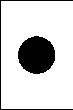
\includegraphics[width=0.5cm]{../latex/assets/insets/spherical.pdf}};
						\end{axis}
					\end{tikzpicture}
				}
			\end{figure}
		\end{frame}

		\begin{frame}
			\frametitle{Recommendations}
			\begin{itemize}
				\item \alert{Shear wave speed quantification} yields best results
				\begin{itemize}
					\item Quantifiable
					\item Most accurate
				\end{itemize}
				\item ARFI and shear wave speed quantification are depth-limited (tissue safety)
				\begin{itemize}
					\item Quasi-static elastography for deep ($\gtrsim \SI{5}{\cm}$) regions
				\end{itemize}
				\item Small lesions ($r \lesssim \SI{5}{\mm}$) are difficult to detect
				\begin{itemize}
					\item MRI-acquired lesions generally have $r \gtrsim \SI{1}{\cm}$
				\end{itemize}
				\item Complicated geometries can affect results
				\item Future work should involve \alert{animal} and \alert{human} studies
				\begin{itemize}
					\item This is the first stage in employing ultrasound elastography as a clinical deep tissue injury detection mechanism
				\end{itemize}
			\end{itemize}
		\end{frame}
		
		\begin{frame}
			\frametitle{Thank-You}
			\vspace{1cm}
			Thank-you to my supervisors, \alert{Dr. Walied Moussa} and \alert{Dr. Martin Ferguson-Pell} for their guidance, my labmates for support, and the Project SMART team for funding and support.
			\vspace{1cm}
			\begin{figure}
				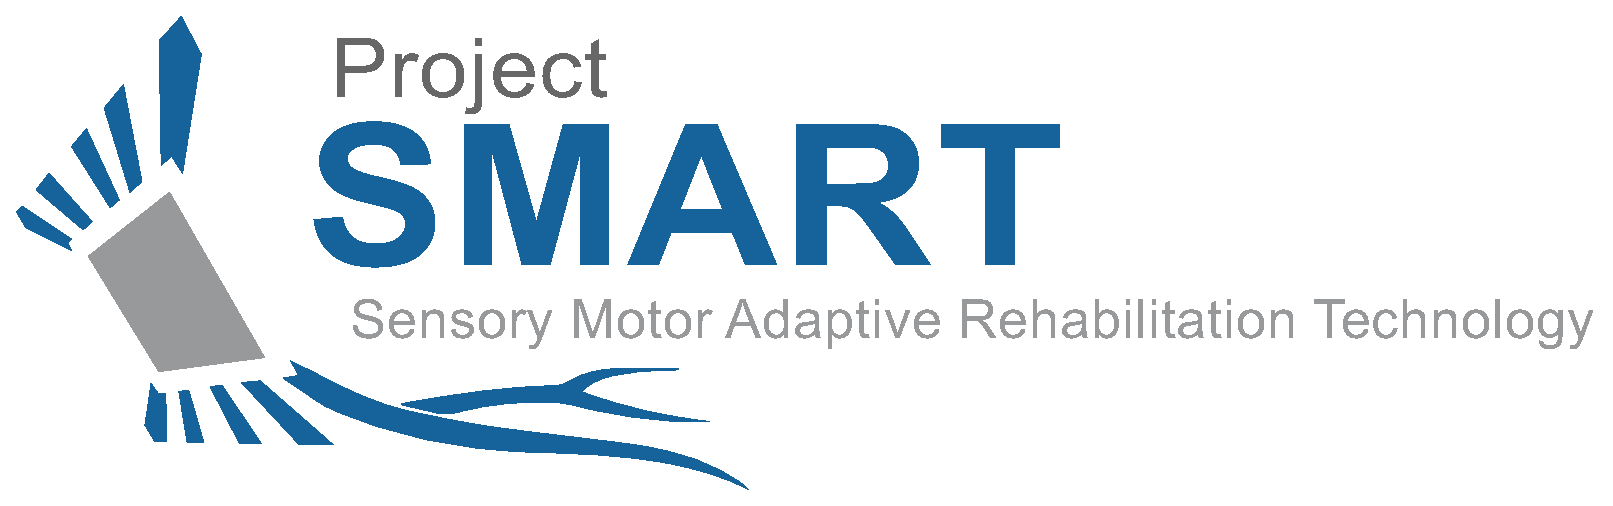
\includegraphics[width=\textwidth]{assets/SMART.eps}
			\end{figure}
		\end{frame}

	\AtBeginSection{}
	\appendix
	\section{Additional Slides}
	\setcounter{showProgressBar}{0}
	\setcounter{showSlideNumbers}{0}

		\begin{frame}
			\frametitle{Additional Slides}
			\begin{itemize}
				\item \hyperlink{refs}{References}
				\item \hyperlink{experimentalSetup}{Experimental Setup}
				\item \hyperlink{arfiForceDerivation}{Derivation of ARFI}
				\item \hyperlink{qsParameters}{Quasi-Static Parameters}
				\item \hyperlink{arfiParameters}{ARFI Parameters}
				\item \hyperlink{shearParameters}{Shear Parameters}
				\item \hyperlink{cirsProperties}{Phantom Properties}
			\end{itemize}
		\end{frame}

		\begin{frame}[allowframebreaks]
			\frametitle{References}
			\label{refs}
			\bibliographystyle{IEEEtran}
			\bibliography{../latex/references.bib}
		\end{frame}

		\begin{frame}[label=experimentalSetup]
			\frametitle{Experimental Setup}
			\begin{center}
				\begin{figure}
					\centering
					\begin{tikzpicture}
						\node at (0, 0) {\includegraphics[width=0.9\textwidth]{../latex/assets/experimental_setup.png}};

						% the phantom
						\draw[pc3,->,ultra thick] (-0.5, 1) -- (-1,-0.6);
						\draw (-0.5, 0.5) node[above,text width=1in,align=center,fill=white,rounded corners=3pt,draw=pc3,ultra thick]{\color{black}\footnotesize CIRS Elasticity QA Phantom model 049};

						% the probe
						\draw[pc2,->,ultra thick] (-2, -2.5) -- (0, -1);
						\draw (-2, -2.5) node[below,text width=1in,align=center,fill=white,rounded corners=3pt,draw=pc2,ultra thick]{\color{black}\footnotesize 9L4 Transducer};

						% the ultrasound machine
						\draw[pc1,->,ultra thick] (-0.75, 3) -- (2.5, 2.15);
						\draw (-0.5, 3) node[left,text width=1.5in,align=center,fill=white,rounded corners=3pt,draw=pc1,ultra thick]{\color{black}\footnotesize Siemens ACUSON S2000\textsuperscript{\texttrademark}\ portable ultrasound machine};
					\end{tikzpicture}
				\end{figure}
			\end{center}
		\end{frame}

		\begin{frame}[label=arfiForceDerivation]
			\frametitle{Derivation of Acoustic Force}
			\begin{columns}[c]
				\column{0.5\textwidth}
					\begin{equation*}
						\label{equ:arfi_linear_momentum}
						\sigma_{ij,j} + \rho b_i = \rho f_i
					\end{equation*}
					\begin{equation*}
						\label{equ:radiation_force_1a}
						\vec{F} = \nabla p_2 - \mu_{tissue} \nabla^2 \vec{v_2}
					\end{equation*}
					\begin{equation*}
						\label{equ:radiation_force_1b}
						\vec{F} = \rho \langle\vec{v_1}\nabla\cdot\vec{v_1} + \vec{v_1}\nabla\vec{v_1}\rangle 
					\end{equation*}
					\begin{equation*}
						\label{equ:radiation_force_2}
						\vec{F} = 2\rho\langle \vec{v} \vec{v}_{,x} \rangle
					\end{equation*}
					\begin{equation*}
						\label{equ:particle_velocity}
						\vec{v} = i\omega A e^{-\alpha x + i\left(\omega t - k x\right)}\hat{x}
					\end{equation*}
					\begin{equation*}
						\label{equ:radiation_force_3}
						\left|\vec{F}\right| = A^2 e^{-2\alpha x}\rho\alpha
					\end{equation*}
					\begin{equation*}
						\label{equ:radiation_force}
						\boxed{\left|\vec{F}\right| = \frac{2\alpha I}{c}}
					\end{equation*}

				\column{0.5\textwidth}
					\begin{center}
						\begin{tabular}{ll}
							$\langle\rangle$: & Time-average \\
							$\vec{F}$: & Acoustic Force \\
							$\vec{v}$: & Particle velocity \\
							$\rho$: & Tissue density \\
							$\alpha$: & Absorption coefficient \\
							$I$: & Acoustic intensity \\
							$c$: & Speed of sound \\
						\end{tabular}
					\end{center}
			\end{columns}
		\end{frame}

		\begin{frame}[label=qsParameters]
			\frametitle{QS USE Parameters}
			\centering
			\scriptsize
			\begin{tabular}{lccs[table-unit-alignment = left]}
				\toprule
				Parameter & Symbol & Values & Units \\
				\midrule
				Lesion depth & $d$ & \numlist{3.5;6.5;8.5;10.0} & \si{\cm} \\
				Lesion altitude & $h$ & \numlist{1.25;2.50;3.75} & \si{\cm} \\
				Lesion diameter & $\diameter S$ & \numlist{0.5;1.0;2.0;2.5} & \si{\cm} \\
				Lesion stiffness ratio & $E_{rel}$ & \numlist{0.32;0.56;1.80;3.20} & - \\
				Ultrasound frequency & $f$ & \numlist{2;4;8} & \si{\MHz} \\
				Transducer-applied strain & $\varepsilon_{app}$ & \numlist{2.5;5.0;10.0} & \si{\percent} \\
				Co-located separation distance & $\delta_{sep}$ & \numlist{1.25;1.50;1.75;2.00} & \si{\cm} \\
				Blurred lesion blur radius & $b_r$ & \numlist{1.0;2.5;5.0;7.5} & \si{\mm} \\
				Clustered lesion density & $b_\rho$ & \numlist{10;20;30;40} & \si{\per\cm\squared} \\
				Clustered lesion radius & $r_{bl}$ & \numlist{0.5;1.0;1.5} & \si{\mm} \\
				Visible human lesion width & $\diameter L$ & \numlist{0.5;1.0;2.0;2.5} & \si{\cm} \\
				Visible human lesion depth & $d$ & \numlist{6.25;6.75;7.25} & \si{\cm} \\
				\bottomrule
			\end{tabular}
		\end{frame}

		\begin{frame}[allowframebreaks,label=arfiParameters]
			\frametitle{ARFI Parameters}
			\centering
			\scriptsize
			\begin{tabular}{llSs[table-unit-alignment = left]}
				\toprule
				Property & Symbol & {Value} & Units \\
				\midrule
				Nonlinearity parameter & $\sfrac{B}{A}$ & 8 & - \\
				Power law prefactor & $\alpha_0$ & 0.7 & $\si{\neper} \left(\si{rad\per\s}\right)^{-y} \si{\per\m}$ \\
				Power law exponent & $y$ & 0.95 & - \\
				Density & $\rho_0$ & 1060 & \si{\kg\per\m\cubed} \\
				\bottomrule
			\end{tabular}
		\end{frame}

		\begin{frame}
			\frametitle{ARFI Parameters}
			\centering
			\scriptsize

			\begin{tabular}{llSs[table-unit-alignment = left]}
				\toprule
				Property & Symbol & {Value} & Units \\
				\midrule
				Bulk Modulus & $K$ & 515.7 & \si{\kPa} \\
				Shear Modulus & $\mu_{tissue}$ & 1.0 & \si{\kPa} \\
				Density & $\rho$ & 1060 & \si{\kg\per\m\cubed} \\
				\bottomrule
			\end{tabular}
			\vspace{1cm}
			\begin{tabular}{SSS}
				\toprule
				{Branch} & {Shear Modulus} & {Relaxation Time} \\
				& {(\si{\Pa})} & {(\si{\s})} \\
				\midrule
				1 & 791.0 & 2 \\
				2 & 66.5 & 40 \\
				3 & 0.6 & 80 \\
				\bottomrule
			\end{tabular}
		\end{frame}

		\begin{frame}
			\frametitle{ARFI Parameters}
			\centering
			\scriptsize

			\begin{tabular}{lccs[table-unit-alignment = left]}
				\toprule
				Parameter & Symbol & Values & {Units} \\
				\midrule
				ARFI interrogation frequency & $f$ & \numlist{1;2;4;6} & \MHz \\
				Transducer width & $w_{trans}$ & \numlist{4;8;10} & \cm \\
				ARFI pulse cycles & $n_c$ & \numlist{3;100;300;500;700} & - \\
				ARFI source pressure & $P_{source}$ & \numlist{4;5;6;7;8} & \MPa \\
				Lesion depth & $d$ & \numlist{1;2;3;4;5;6;7;8;9} & \cm \\
				Lesion diameter & $\diameter S$ & \numlist{0.5;1.0;2.0;2.5} & \cm \\
				Lesion stiffness ratio & $E_{rel}$ & \numlist{0.32;0.56;1.80;3.20} & - \\
				Blurred lesion blur radius & $b_r$ & \numlist{1.0;2.5;5.0;7.5} & \mm \\
				Clustered lesion density & $b_\rho$ & \numlist{10;20;30;40} & \per\cm\squared \\
				Clustered lesion radius & $r_{bl}$ & \numlist{0.5;1.0;1.5} & \mm \\
				Visible human lesion width & $\diameter L$ & \numlist{0.5;1.0;2.0;2.5} & \cm \\
				\bottomrule
			\end{tabular}
		\end{frame}

		\begin{frame}[label=shearParameters]
			\frametitle{Shear Parameters}
			\centering
			\scriptsize

			\begin{tabular}{lccs[table-unit-alignment = left]}
				\toprule
				Parameter & Symbol & Values & Units \\
				\midrule
				Lesion depth & $d$ & \numlist{1;2;3;4;5;6;7;8;9} & \si{\cm} \\
				Lesion diameter & $\diameter S$ & \numlist{0.5;1.0;2.0;2.5} & \si{\cm} \\
				Lesion offset & $d_{off}$ & \numlist{0.00;1.25;2.50;3.75} & \si{\cm} \\
				Lesion stiffness ratio & $E_{rel}$ & \numlist{0.32;0.56;1.80;3.20} & \\
				Blurred lesion blur radius & $b_r$ & \numlist{1.0;2.5;5.0;7.5} & \si{\mm} \\
				Clustered lesion density & $b_\rho$ & \numlist{10;20;30;40} & \si{\per\cm\squared} \\
				Clustered lesion radius & $r_{bl}$ & \numlist{0.5;1.0;1.5} & \si{\mm} \\
				Visible human lesion width & $\diameter L$ & \numlist{0.5;1.0;2.0;2.5} & \si{\cm} \\
				\bottomrule
			\end{tabular}
		\end{frame}

		\begin{frame}[label=cirsProperties]
			\frametitle{CIRS Phantom Properties}
			\centering
			\scriptsize
			\begin{tabular}{lccs[table-unit-alignment = left]}
				\toprule
				Property & Symbol & Value & Units \\
				\midrule
				Nominal basal elastic modulus & $E_{tissue}$ & 25 & \si{\kPa} \\
				Lesion elastic modulus & $E_{lesion}$ & \numlist{8;14;45;80} & \si{\kPa} \\
				Speed of sound & $c_0$ & 1540 & \si{\metre\per\second} \\
				Acoustic attenuation & $\alpha$ & 0.5 & \si{\decibel\per\cm\per\MHz} \\
				Lesion diameter & $\diameter S$ & \numlist{10;20} & \si{\mm} \\
				Lesion depth & $d$ & \numlist{15;35} & \si{\mm} \\
				\bottomrule
			\end{tabular}
		\end{frame}

\end{document}